\documentclass{article}
\usepackage{geometry}
\usepackage{amsmath}
\usepackage{titling}
\usepackage{graphicx}
\usepackage{hyperref}

\hypersetup{colorlinks=true,urlcolor=cyan,linkcolor=blue}

\pretitle{\begin{center}\huge}
\posttitle{\end{center}}
\preauthor{\begin{center}\small}
\postauthor{\end{center}}
\predate{\begin{center}\footnotesize}
\postdate{\end{center}}
\setlength{\droptitle}{-40pt}

\title{Probe hardware and software updates}
\date{February, 2022}
\author{Brian Frost}
\begin{document}

\maketitle

\section{Introduction}

\par{A spectral domain optical coherence tomography probe (hereafter ``the probe") was designed by Nathan Lin, and is presented in his PhD thesis. While his preliminary work validated the functionality of this probe, a significant amount of work has been done since his departure to improve the probe's functionality.}
\par{In particular, I have worked at improving the probe's accessibility, allowing for better interfacing with the ThorImage software, and for real-time B-Scanning at higher quality than what ThorImage produces. I have also produced acquisition software that allows us to process probe-acquired data using the exact same pipeline as standard bulk-optics-acquired data.}
\par{In this document, I will discuss these advancements at a high level, giving significant detail for new features and leaving older features to previous documentation found on \href{https://github.com/Brian-Frost-LaPlante/LabReports}{my GitHub page}. In particular, for information on the probe, see the \href{https://github.com/Brian-Frost-LaPlante/LabReports/blob/main/ProbeReports/ProbeDriverReport.pdf}{Probe Driver Report}. For excruciating detail on the theory of OCT background subtraction and the acquisition/processing functions for the probe, see the \href{https://github.com/Brian-Frost-LaPlante/LabReports/blob/main/ProbeReports/Fixed-BackgroundProcessing.pdf}{Fixed-Background Processing Report}.}

\par{I will first give a bit of intuition regarding the background used in OCT processing (\hyperlink{bgsection}{Sec. \ref{bgsection}}), specifically as it pertains to use of the ThorImage software. I avoid repetition from my previous report and look only emphasize and explain some phenomena we have recently observed using the probe alongside ThorImage.}
\par{I will continue with an overview of the circuit's functionality (\hyperlink{circsection}{Sec. \ref{circsection}}). I emphasize key changes since the last report was written, and signal qualities that need to be kept in mind when changing between probes.}
\par{I will then discuss updates to the control programs used for acquiring and observing data from the probe (\hyperlink{controlprograms}{Sec. \ref{controlprograms}}). I will also discuss the means by which ThorImage can be used with the probe, and how the data displayed in ThorImage ought to be interpreted (\hyperlink{thorimagesection}{Sec. \ref{thorimagesection}}).}
\par{Finally, I will show some important data taken from the probe which ought to influence how we interpret all future probe-acquired scans. First, we show that the SNR in water is significantly worse than that in air (\hyperlink{SNRsection}{Sec. \ref{SNRsection}}), which is important for \textit{in vivo} experiments where data is taken in the fluid of the cochlea. Lastly, we show an interesting phenomenon wherein despite low SNR, we can achieve informative B-Scans formed of low-quality A-Scans (\hyperlink{BScansection}{Sec. \ref{BScansection}}). We discuss how this fact can be used to extract location information from the time-averaged M-Scan magnitude.}

\section{The background in OCT processing}\label{bgsection}
\hypertarget{bgsection}{}

\par{}

\subsection{Why do we need a background?}

\par{}

\subsection{How does ThorImage capture the background?}

\par{}

\subsection{How do our programs handle the background?}

\par{}

\section{Probe control signals and circuitry}\label{circsection}
\hypertarget{circsection}{}

\par{}

\subsection{Telesto output signal}

\par{}

\subsection{Circuit function and capacitance values}

\par{}

\begin{figure}[!h]
	\centering
	\includegraphics[width=0.4\textwidth]{Data for Probe Writeup/10 kHz.jpg}
	\caption{Response at 10 kHz.}
\end{figure}

\begin{figure}[!h]
	\centering
	\includegraphics[width=0.4\textwidth]{Data for Probe Writeup/28 kHz.jpg}
	\caption{Response at 28 kHz.}
\end{figure}

\begin{figure}[!h]
	\centering
	\includegraphics[width=0.4\textwidth]{Data for Probe Writeup/76 kHz.jpg}
	\caption{Response at 76 kHz.}
\end{figure}

\subsection{Adjusting resistances for each probe}

\par{}

\begin{figure}[!h]
	\centering
	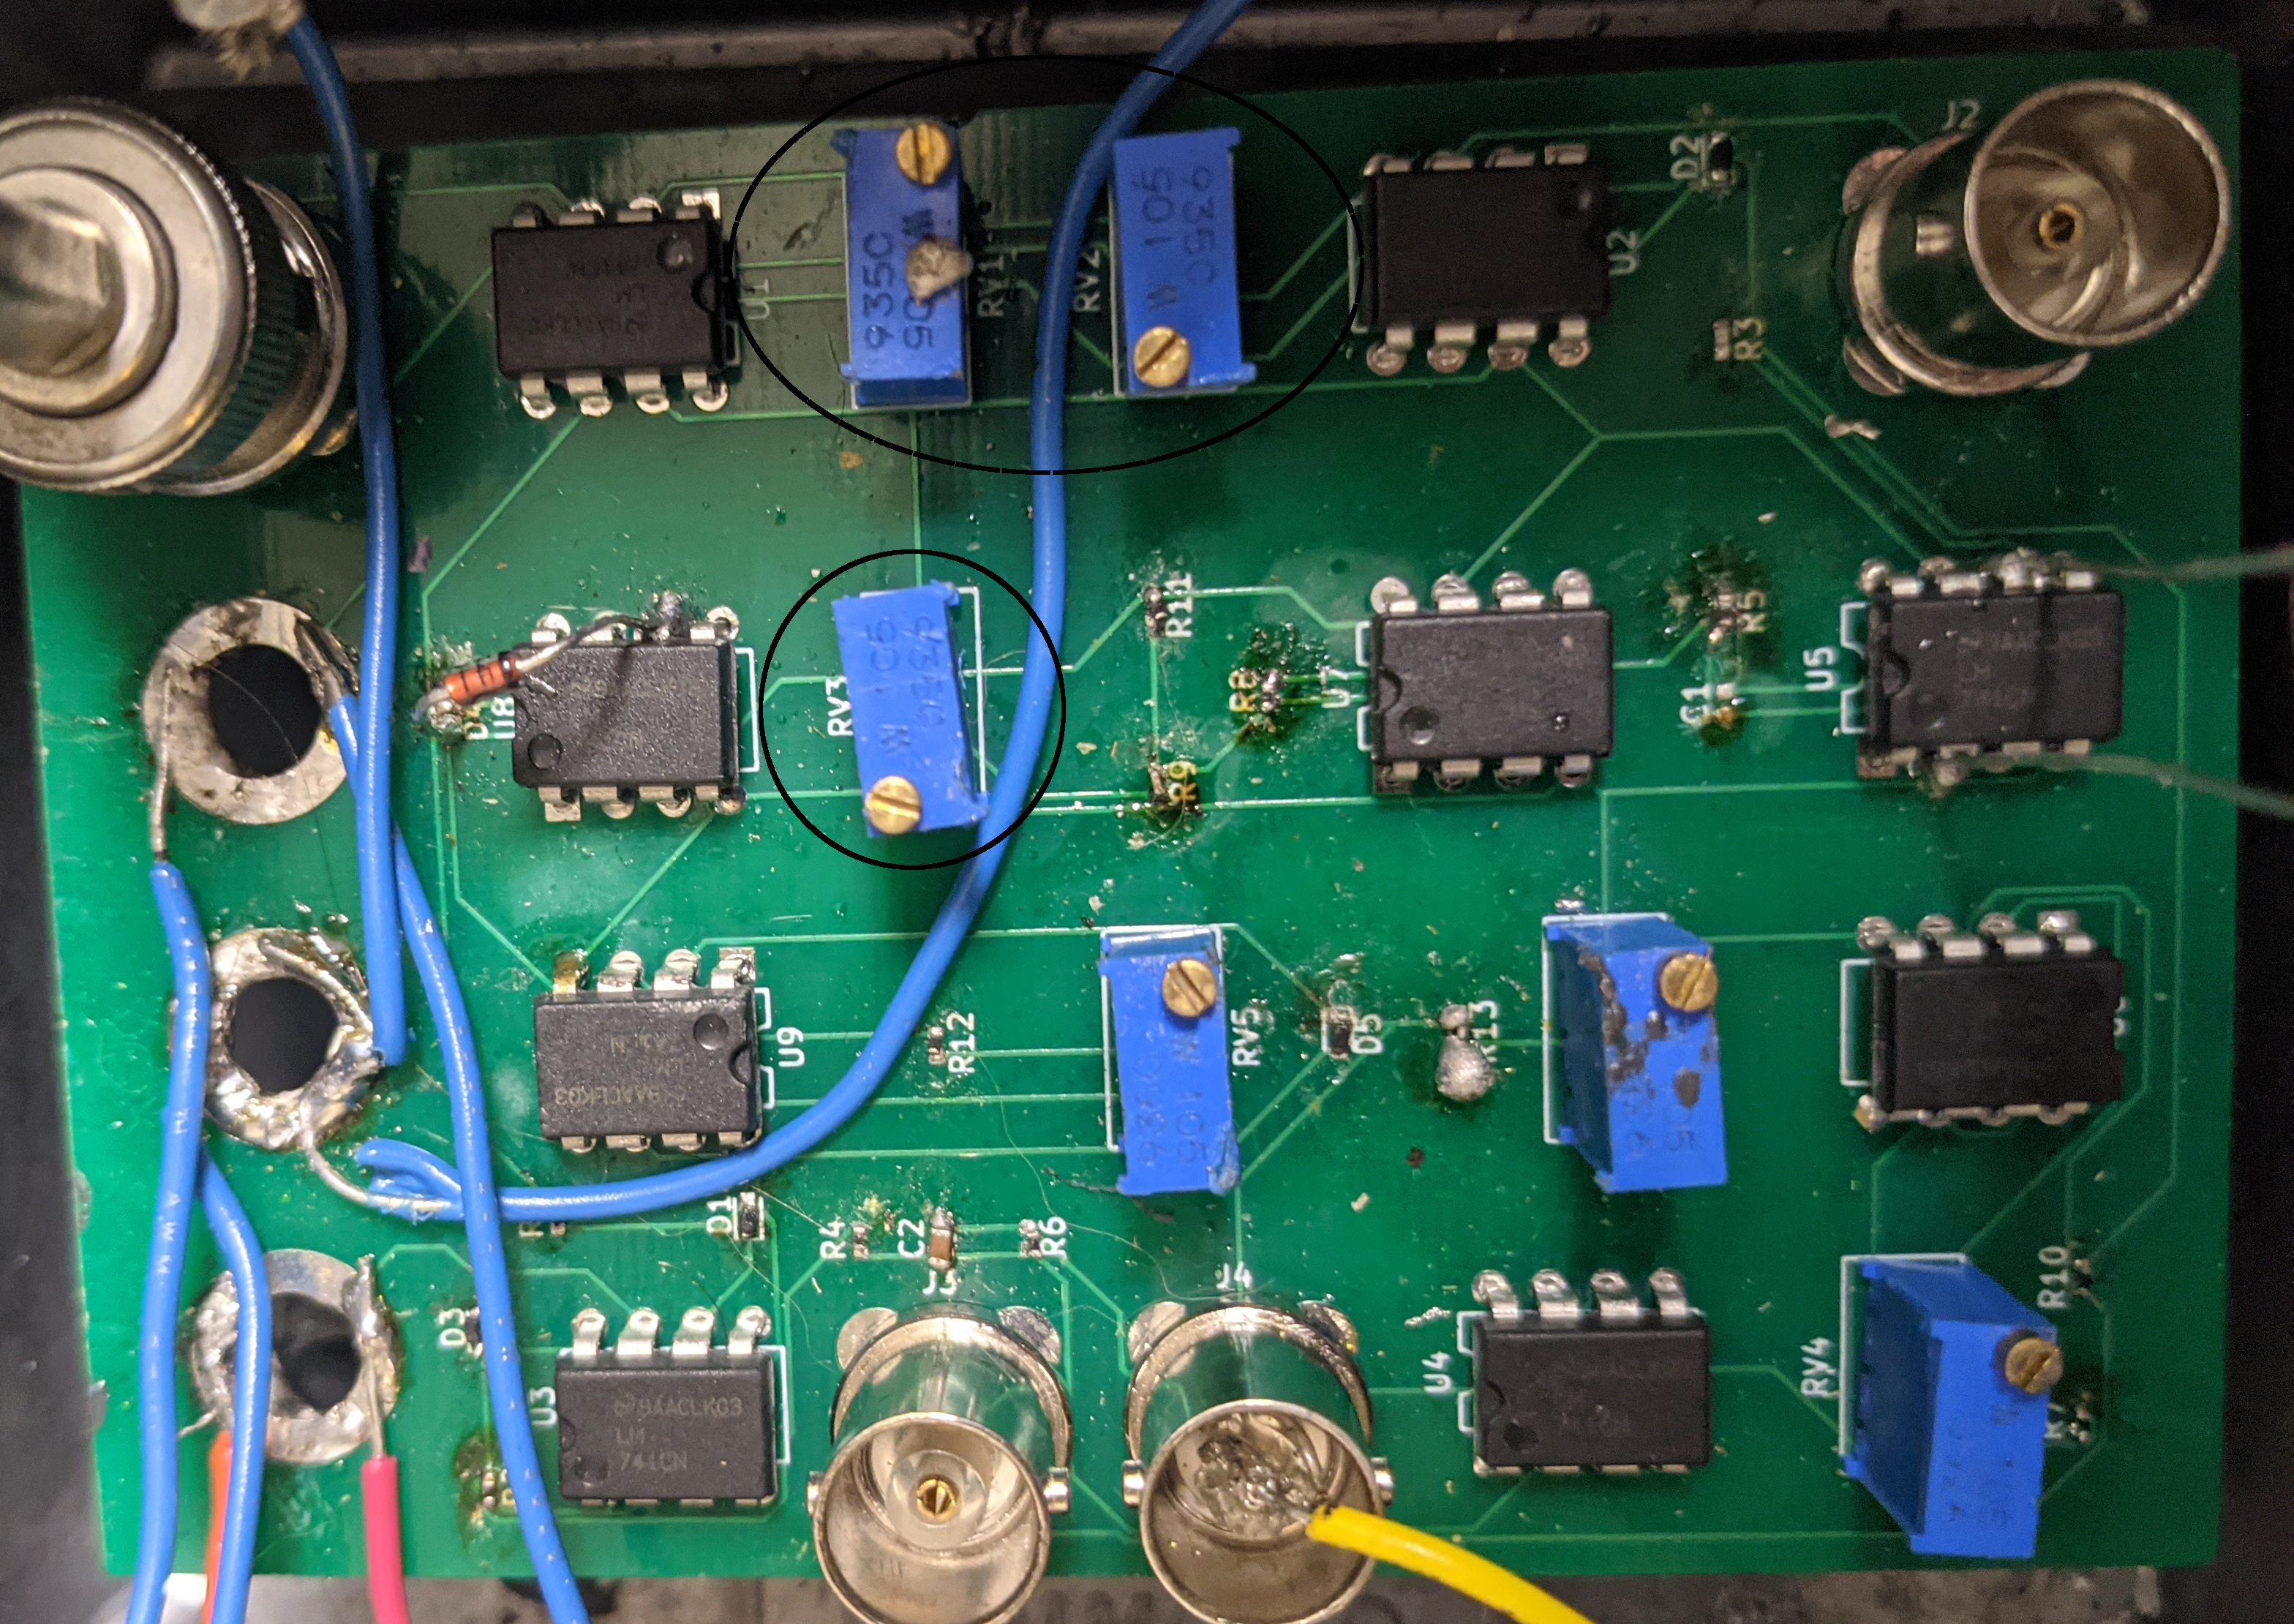
\includegraphics[width=0.6\textwidth]{Data for Probe Writeup/circuit.jpg}
	\caption{Response at 76 kHz.}
\end{figure}

\section{Control programs for fixed background}\label{controlprograms}
\hypertarget{controlprograms}{}

\par{}

\begin{figure}[!h]
	\centering
	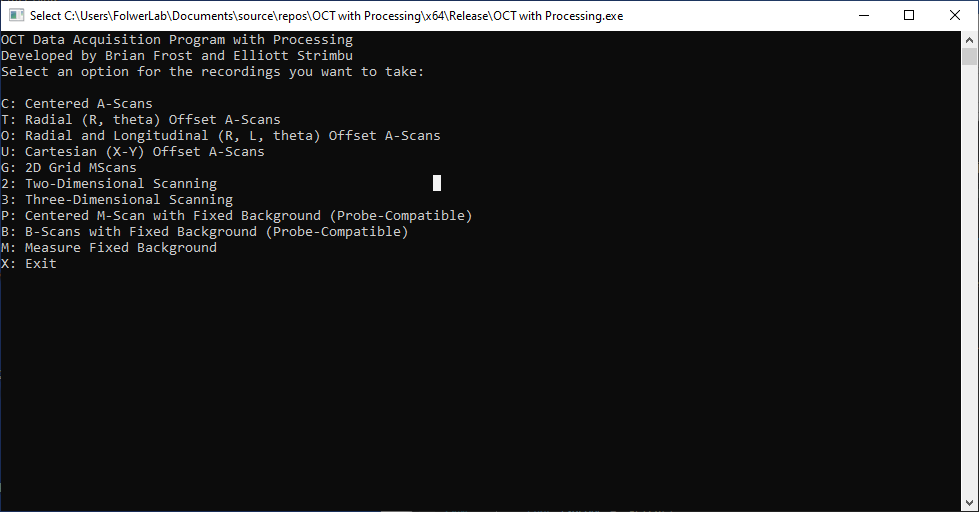
\includegraphics[width=0.6\textwidth]{Data for Probe Writeup/Terminal at Startup.png}
	\caption{.}
\end{figure}

\subsection{Option M: Measure Background}

\par{}

\begin{figure}[!h]
	\centering
	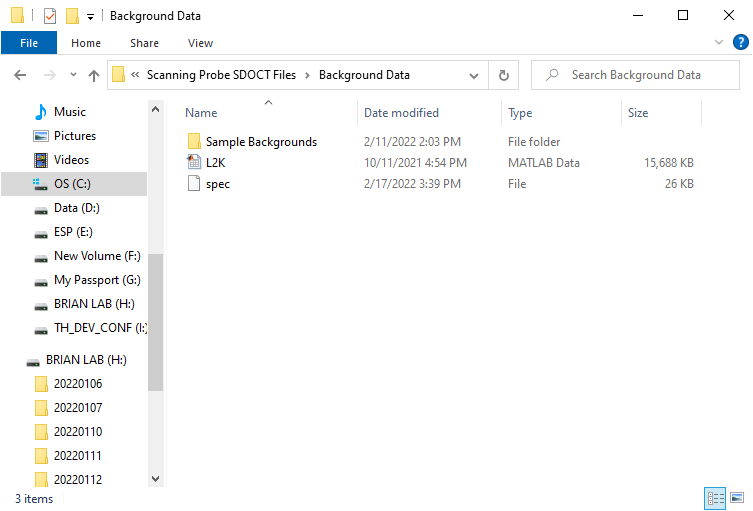
\includegraphics[width=0.6\textwidth]{Data for Probe Writeup/spec location.png}
	\caption{.}
\end{figure}

\subsection{Taking and observing B-Scans with fixed background}

\par{}

\begin{figure}[!h]
	\centering
	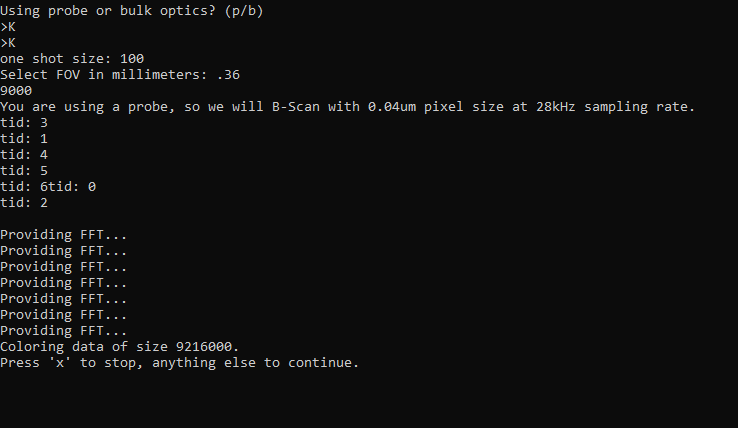
\includegraphics[width=0.6\textwidth]{Data for Probe Writeup/BMode Probe.png}
	\caption{.}
\end{figure}

\begin{figure}[!h]
	\centering
	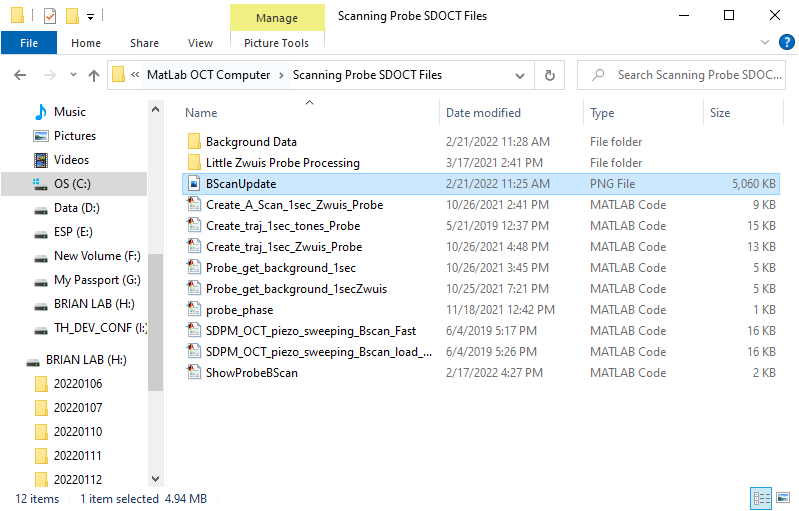
\includegraphics[width=0.6\textwidth]{Data for Probe Writeup/BScan location.png}
	\caption{.}
\end{figure}

\begin{figure}[!h]
	\centering
	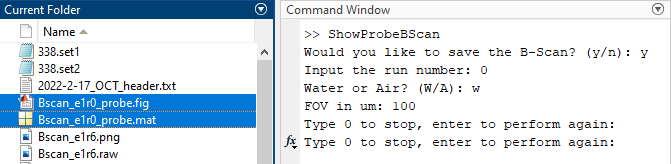
\includegraphics[width=0.6\textwidth]{Data for Probe Writeup/ShowProbeBScan operation.png}
	\caption{.}
\end{figure}

\begin{figure}[!h]
	\centering
	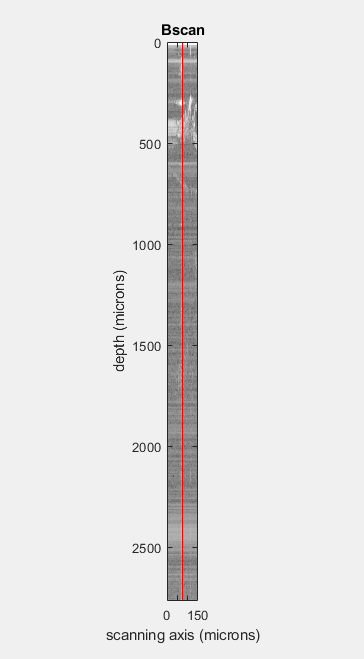
\includegraphics[width=0.6\textwidth]{Data for Probe Writeup/BScan fig update.png}
	\caption{.}
\end{figure}

\subsection{Option P: M-Scans with fixed background}

\par{}

\section{Using ThorImage with the probe}\label{thorimagesection}
\hypertarget{thorimagesection}{}

\par{}


\begin{figure}[!h]
	\centering
	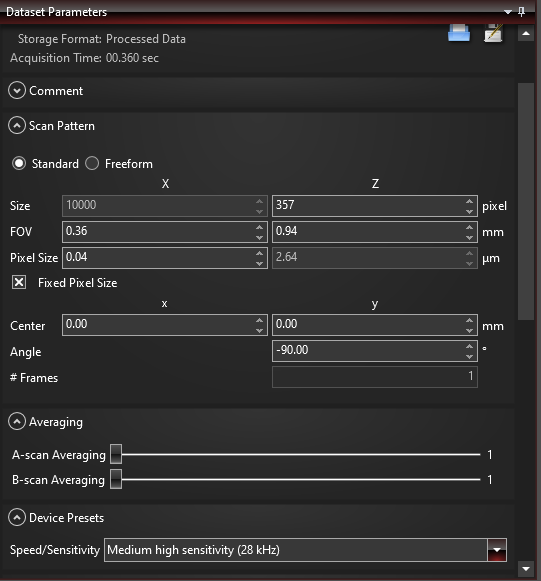
\includegraphics[width=0.6\textwidth]{Data for Probe Writeup/ThorImage settings for BScan.png}
	\caption{.}
\end{figure}


\subsection{The ThorImage ``fake background" trick}

\par{}

\section{Signal quality}

\par{}

\subsection{SNR in air vs. water}\label{SNRsection}
\hypertarget{SNRsection}{}

\par{}

\begin{figure}[!h]
	\centering
	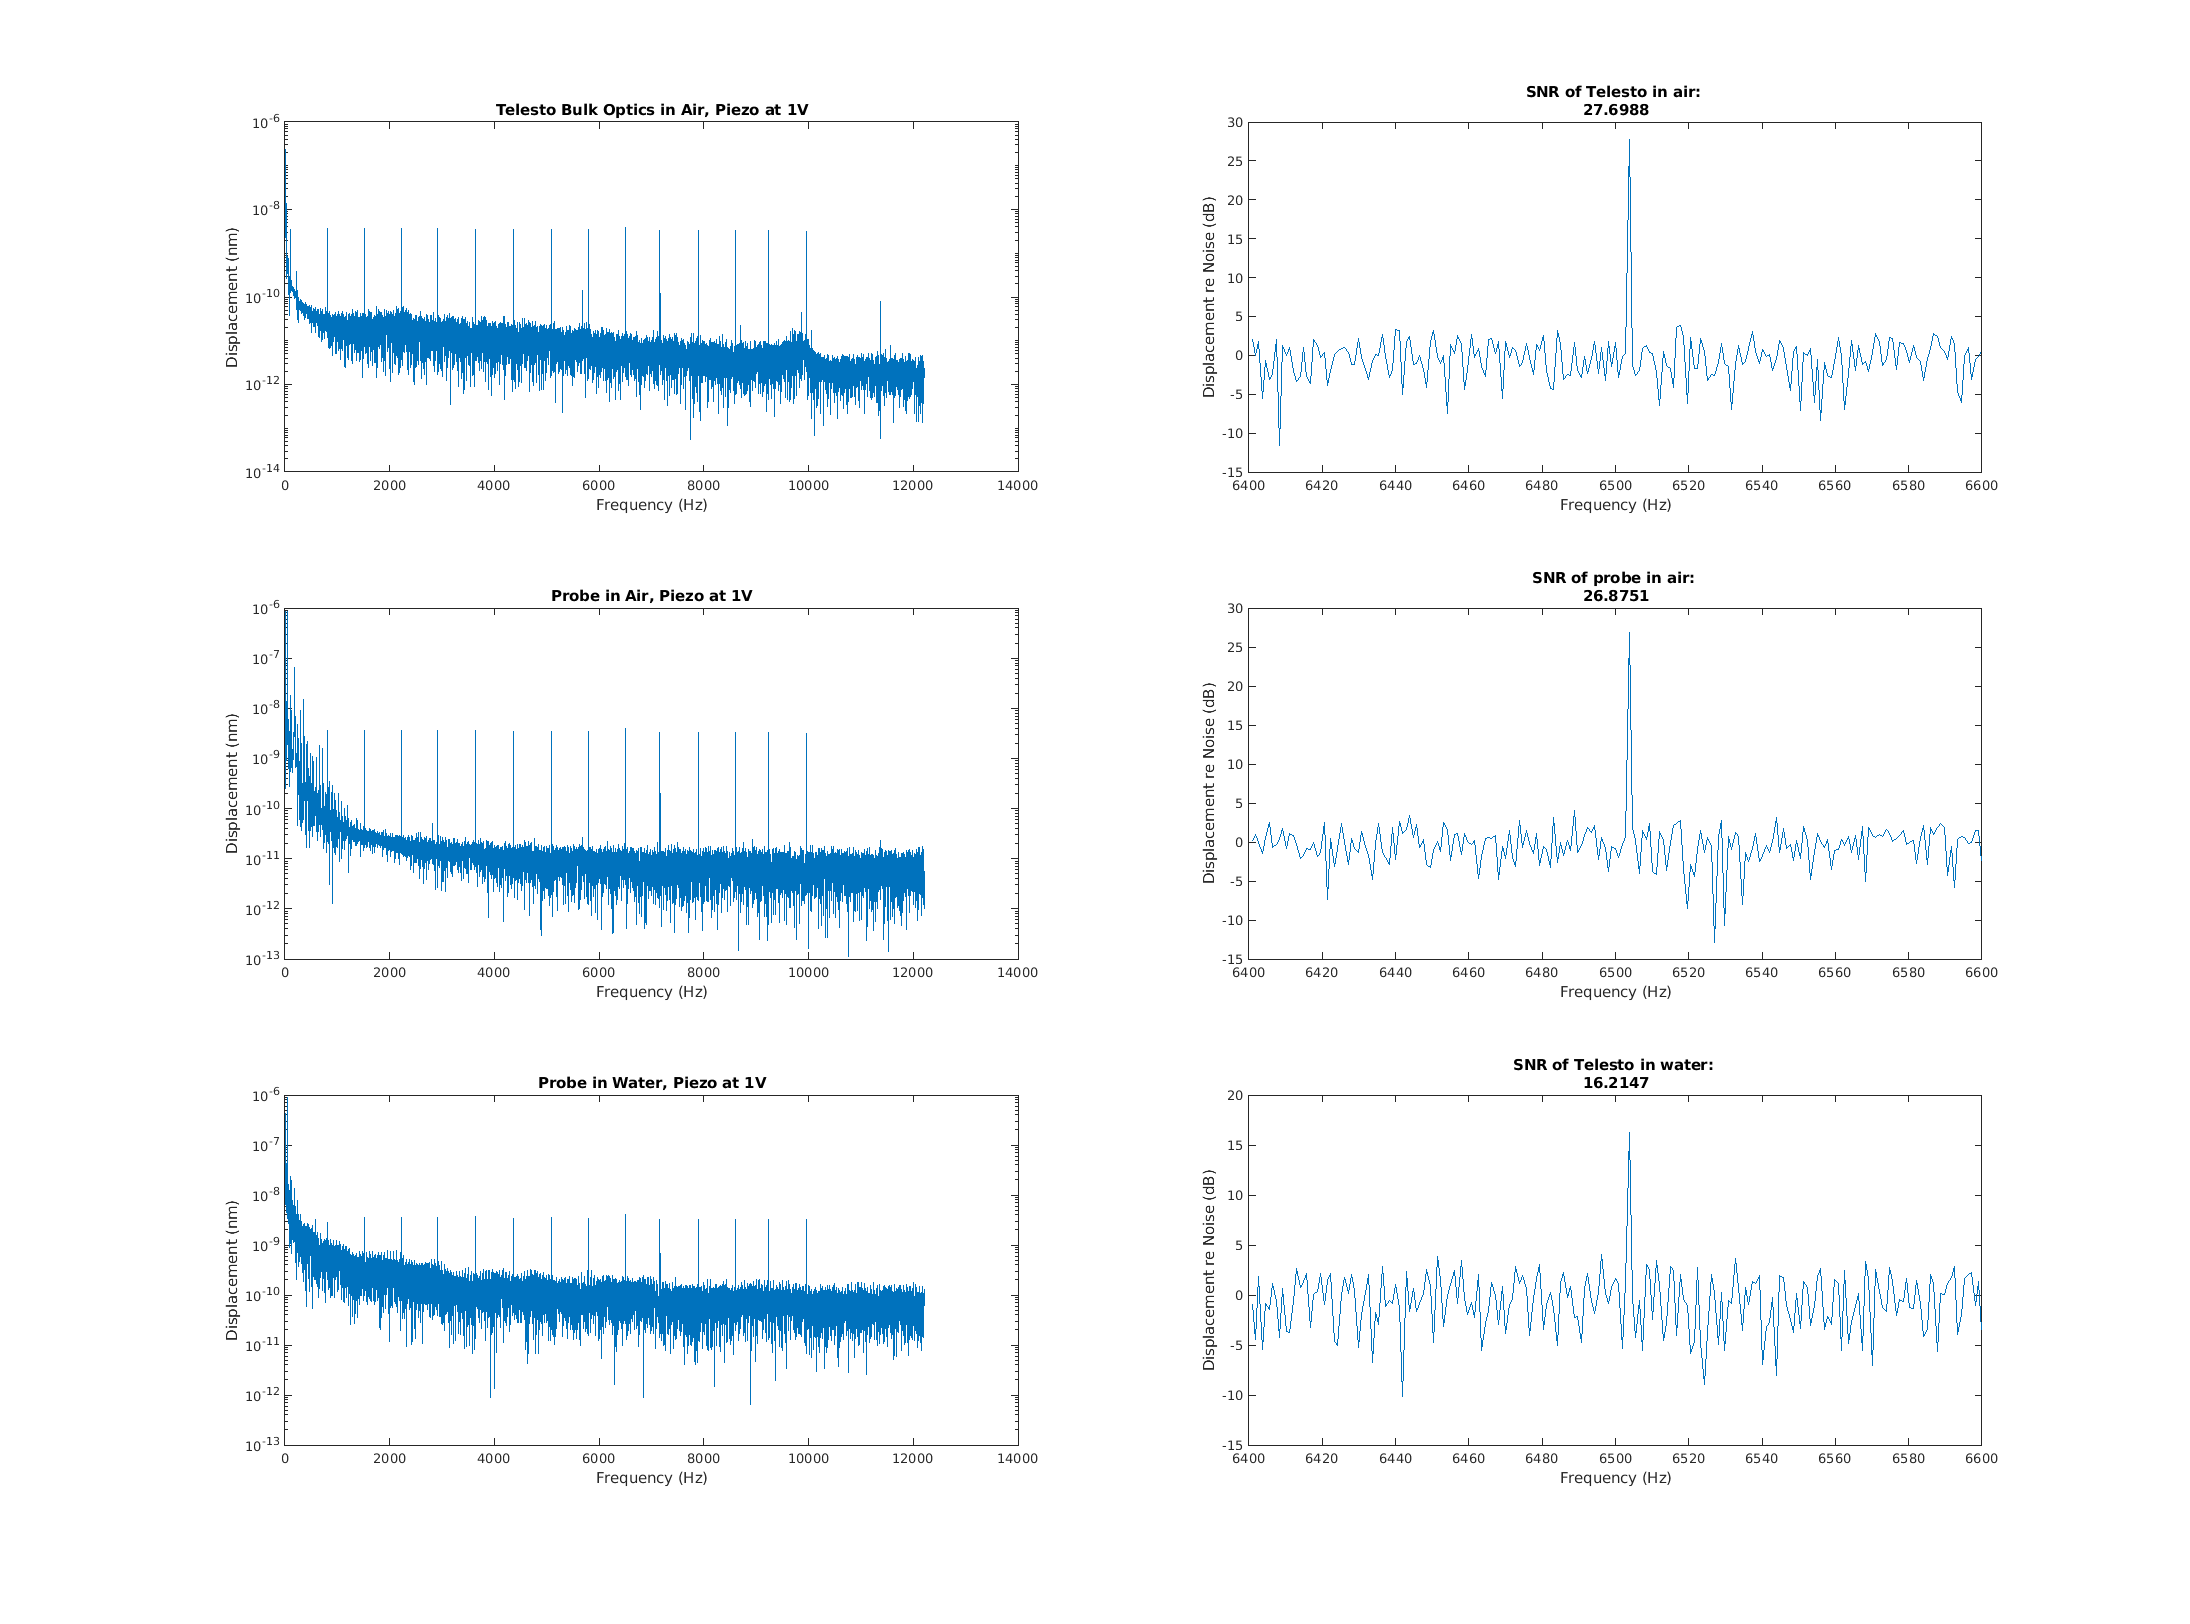
\includegraphics[width=\textwidth]{Data for Probe Writeup/SNRcomp.png}
	\caption{.}
\end{figure}

\subsection{B-Scan quality}\label{BScansection}
\hypertarget{BScansection}{}

\par{}

\begin{figure}[!h]
	\centering
	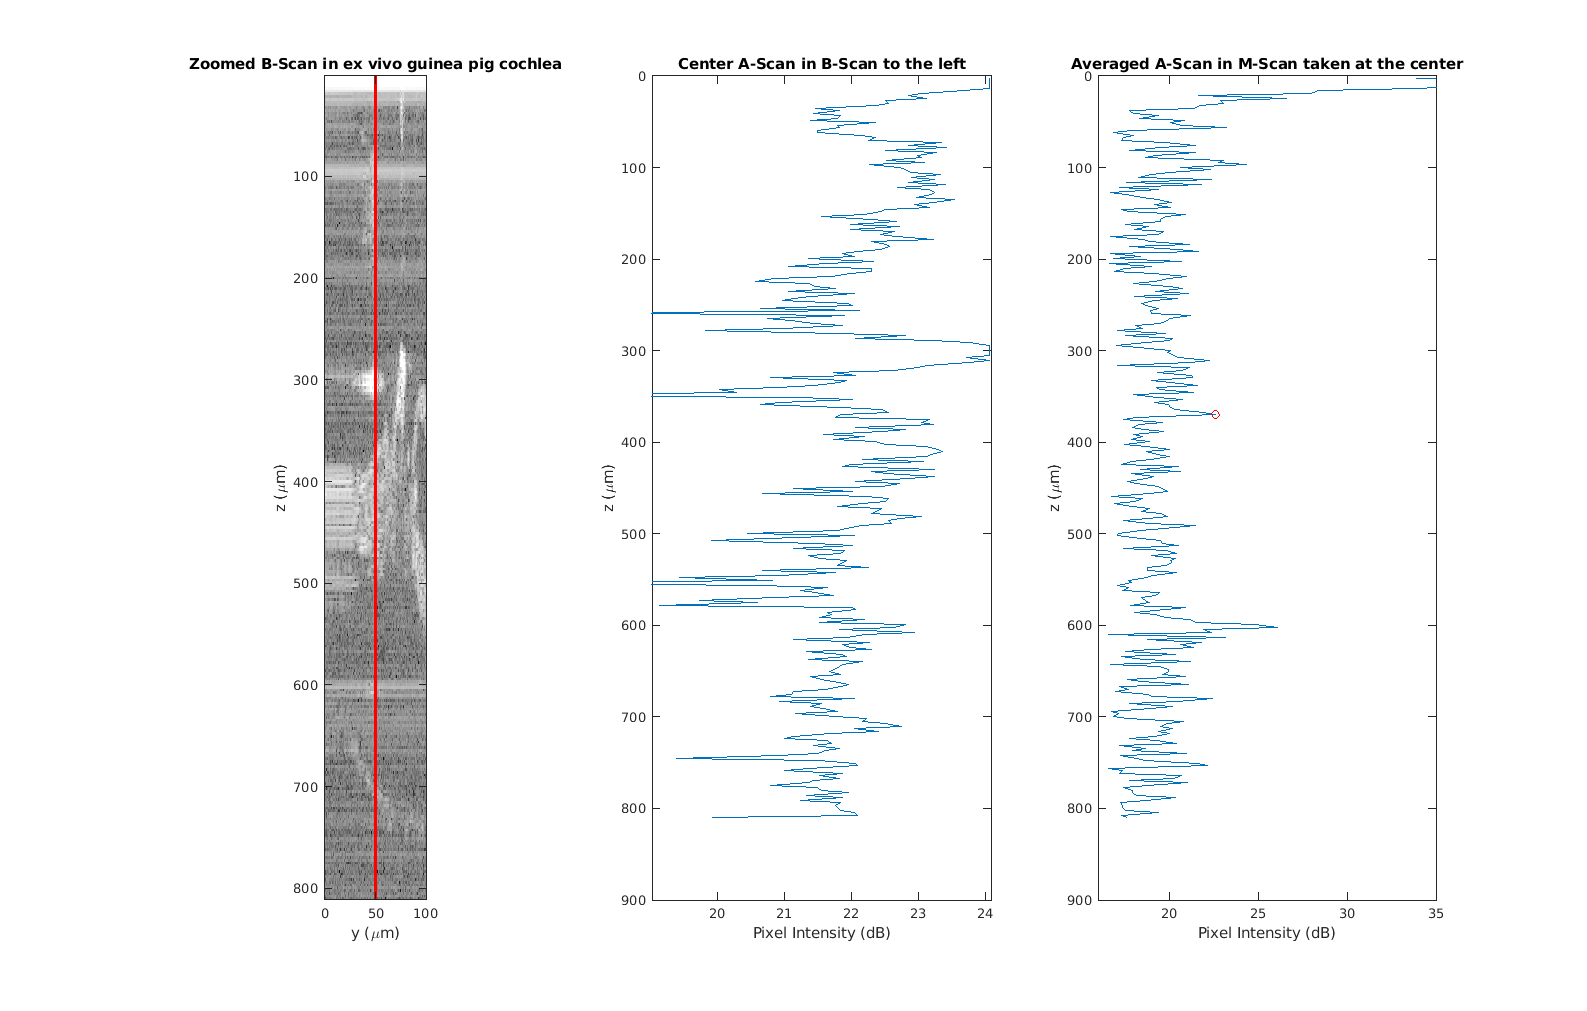
\includegraphics[width=\textwidth]{Data for Probe Writeup/Data 2022-2-17/BScan v AScan.png}
	\caption{.}
\end{figure}


\end{document}
